\documentclass{report}
\usepackage{pgf}
\usepackage{tikz}
\usepackage{verbatim}
\usepackage{url}
\usepackage{hyperref}	% Clickable links to figures, references and urls.

\usepackage{graphicx}

\begin{document}

\title{Automated Worm Fingerprinting}
\author{Awais Aslam \and Attique Dawood}
\maketitle

\tableofcontents

\begin{abstract}
Worms propagate by contacting vulnerable hosts and infecting them with malicious payload.
The destination address space for such attacks would be large. In case of a worm outbreak
number of infected hosts will grow over time. Some part of worm attack patterns are always
invariant. Such invariant content can be used as worm signatures by analyzing the frequency
at which this content appears in network traffic and the variance in source and destination
addresses. We present an implementation of this method for detecting worms based on the
EarlyBird prototype~\cite{DBLP:conf/osdi/SinghEVS04}.
\end{abstract}

\chapter{Introduction}
\section{Network Intrusion Detection Systems}

Intrusion detection systems monitor network traffic to detect malicious activities. Malicious activities can be an outside attempt to gain control of a host, a worm spreading across the internet or suspicious traffic from a local host etc.

\section{Types of IDS}

IDS are basically either signature--based or anomaly--based. Signature--based IDS need to know specific signatures of malicious content (specific strings or code) beforehand. Anomaly--based IDS identify abnormal patterns in network traffic for detecting suspicious activities.

\section{Automated Signature Generation}

Sumeet et. al.~\cite{DBLP:conf/osdi/SinghEVS04} have presented a method to quickly generate signatures based on anomalous behaviour of worms spreading across the network in order contain them. The method is based on an observation that the probability of unique strings occurring in normal traffic directed to diverse destination is very low.

Intrusion detection techniques used by Snort and Bro rely on vulnerabilities that are well--known by comparing with a database. Automated worm detection assumes that some part of malicious program or code is invariant, i.e. it does not change in order to hide itself. The invariant portion of worm can be used to create signatures since it will occur frequently in network traffic.

The goal of this project is to come up with an efficient implementation of the signature generation algorithm used in EarlyBird prototype.

\chapter{Problem Specification}

\section{Characterizing Worm Behaviour}
Worms are defined as malicious programs that can replicate and spread over the network infecting vulnerable hosts.

Observation of popular worm outbreaks reveal that spreading rate is extremely fast. For example the Slammer worm scanned almost all the internet address space in under 10 minutes~\cite{DBLP:conf/osdi/SinghEVS04}. There is a need to quickly generate signatures in case of a new worm outbreak.

\section{Project Goals}
The goals of this project was to implement an automated worm detection software that can quickly generate worm signatures in order to contain worm activities.

The minimum functionality was to detect already existing worms on the network. In addition, real-time analysis of network traffic requires an efficient implementation to reduce the computational overheads. The program should also be flexible to allow changes in operational parameters in order to tune it for best performance and results.

\chapter{Solution Approach}

\section{Algorithm}
Content Prevalence and Address Dispersion tables keep track of content prevalence and content dispersion. Content prevalence table has two fields for key and count. Address dispersion table has three fields for key, source IP count and destination IP count. Following steps outline the core functionality as depicted in figure~\ref{Algorithm} taken from~\cite{DBLP:conf/osdi/SinghEVS04}:
\begin{enumerate}
\item Network traffic is scanned and keys are generated from packet payloads.
\item If the key is already present in address dispersion table relevant source or destination IP count is incremented. Alarm thresholds are checked in this case.
\item If the key doesn't exist in address dispersion table it is checked in Content prevalence table. If present, content prevalence count is incremented otherwise a new entry is created with count 1. 
\item If the content prevalence count crosses threshold, key is promoted into address dispersion table.
\end{enumerate}

\begin{figure}[here]
\centering
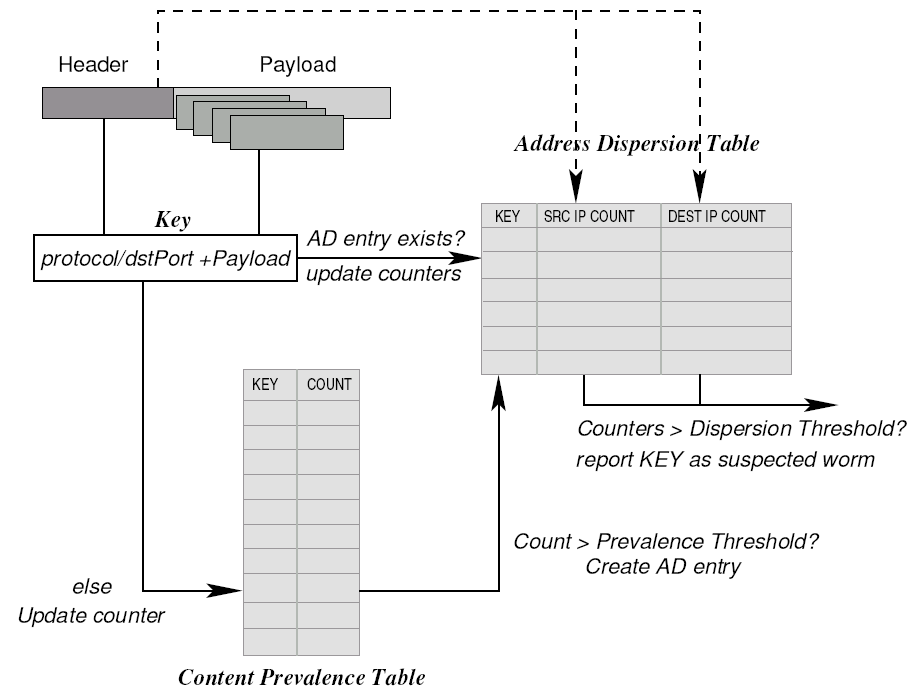
\includegraphics[width=\textwidth]{Algorithm.png}
\caption{Worm detection algorithm}
\label{Algorithm}
\end{figure}

\section{Main Components}
Our implementation is portable and can be run on both Linux or Windows provided the required development libraries are installed. It has the following main components:
\begin{enumerate}
\item Packet capturing section that provides packet payload and header information
\item Packet processing thread to generated keys and index into Content Prevalence and Address Dispersion tables.
\item A garbage collector thread removes any keys from content prevalence table that are outdated.
\item Another thread logs network statistics and dumps any debugging information requested by user.
\end{enumerate}

\chapter{Implementation Details}

\section{Packet Capturing}
On Linux we used the \texttt{libpcap} and for Windows we used the \texttt{winpcap} packet capturing libraries. These libraries are open source projects freely available online.

A filter string needs to be passed as an input argument to the software. This filter string specifies the network traffic to capture. For example, using a filter string ``ip'' will capture all IP packets, similarly a filter string ``TCP\textbar\textbar UDP'' will capture any TCP or UDP packets.

\nocite{*}
\bibliographystyle{ieeetr} %plain, ieeetr
\bibliography{Wormref}

\end{document}




